% ECE4900W Communicating Engineering Solutions
% Author: Arturo Salinas-Aguayo <artjsalina5@uconn.edu>
\documentclass{beamer}
\usetheme{Warsaw}
\usecolortheme{dolphin}
\usefonttheme{professionalfonts}
\setbeamertemplate{navigation symbols}{}
\usepackage{graphicx}
\usepackage{biblatex}
\addbibresource{references.bib}
\graphicspath{{../../images/}}

\title[Safe Nuclear Power]{Safe Nuclear Power: Instrumentation, Human Oversight, and Infrastructure Transition}
\subtitle{ECE 4900W – Summer 2025}
\author[Arturo Salinas]{Arturo Salinas-Aguayo}
\institute[UConn]{University of Connecticut\\College of Engineering}
\date{\today}

\begin{document}

\begin{frame}
  \titlepage
  \speak{Welcome. This presentation explores the technological, ethical, and infrastructural dimensions of nuclear power in the modern world. We will cover lessons from historic accidents, instrumentation, human-machine interface design, and current innovations. Each story reveals both vulnerability and resilience.}
\end{frame}

\begin{frame}{Outline}
  \tableofcontents[pausesections]
  \speak{Here is the roadmap for this presentation. Each section builds on the last, culminating in a call for renewed responsibility and innovation in the nuclear field.}
\end{frame}

\section{Introduction}

\begin{frame}{Motivation}
  \subsubsection*{Why Nuclear Now?}
  \speak{Nuclear energy provides unmatched energy density and emissions-free base-load power. However, public trust and sustainable deployment depend on ethical design, robust control systems, and trained human oversight. While wind and solar depend on weather and batteries, nuclear runs steadily. But one accident can erode decades of progress.}
  \begin{itemize}
    \item Zero-emission base-load power
    \item High energy return on investment
    \item Historical trauma shapes perception \autocite{nrc_chernobyl, worldnuclear_fukushima_review}
    \item Paper focuses on safety through instrumentation and oversight
  \end{itemize}
\end{frame}

\section{Instrumentation and Control}

\begin{frame}{Types of Reactors}
  \subsubsection*{Diverse Architectures}
  \speak{Let’s begin with an overview of reactor types, since their thermal-hydraulic behavior and control logic affect how instrumentation is designed. Each has different challenges.}
  \begin{itemize}
    \item Pressurized Water Reactor (PWR): most common, used in submarines and civilian fleets
    \item Boiling Water Reactor (BWR): direct steam path to turbine
    \item CANDU: heavy water as moderator and coolant
    \item Gas-cooled (AGR): high outlet temperature for efficiency
  \end{itemize}
\end{frame}

\begin{frame}{Instrumentation in a PWR}
  \subsubsection*{Sensor Coverage}
  \speak{This diagram shows typical sensor and actuator placements in a PWR. Note the neutron flux monitors, hot leg thermocouples, pressurizer level gauges, and scram breakers. Each of these is essential for safe operation.}
  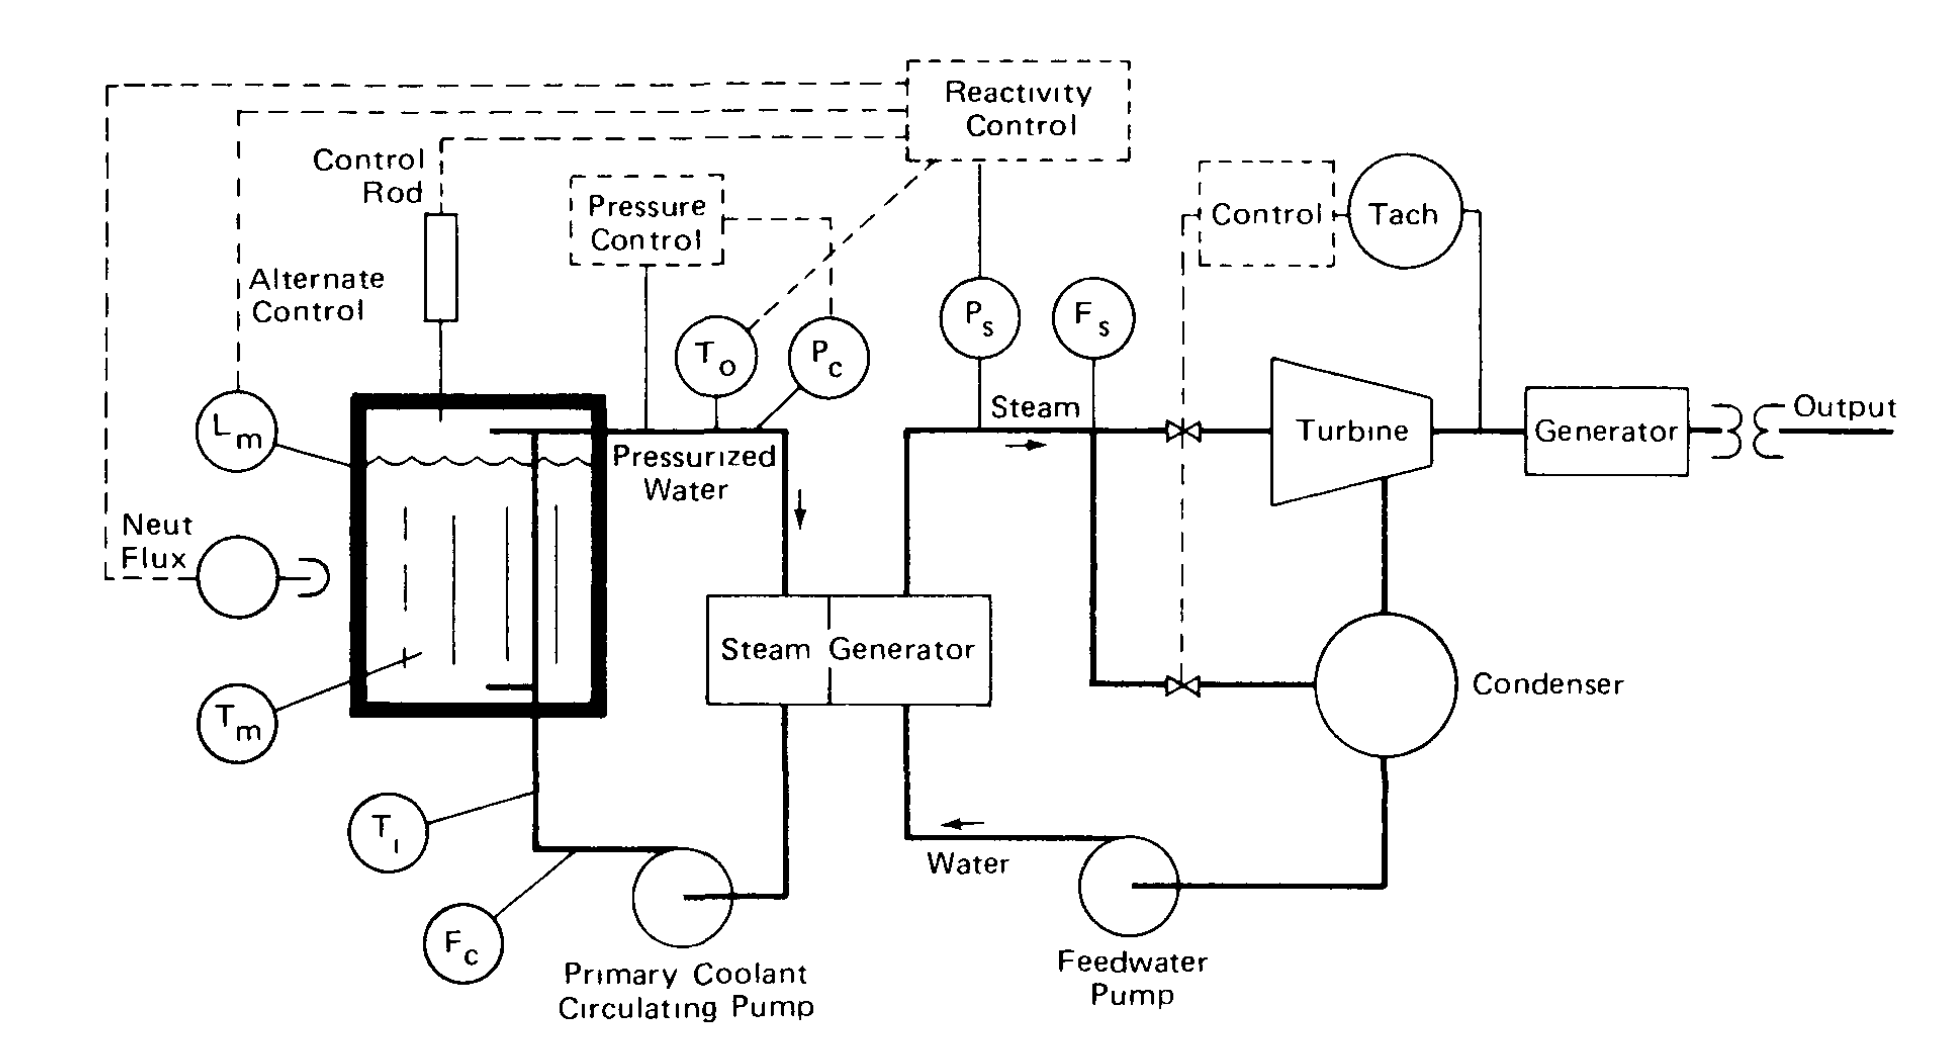
\includegraphics[width=0.85\textwidth]{instrumentation.png}
\end{frame}

\section{Historical Lessons}

\begin{frame}{SL-1: Prompt Critical from Manual Control}
  \subsubsection*{The First Fatal Reactor Accident}
  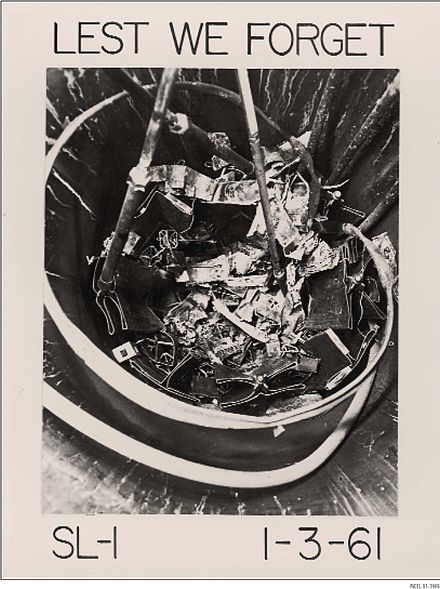
\includegraphics[width=0.4\textwidth]{sl1diagram.jpg}
\end{frame}

\begin{frame}{SL-1: Prompt Critical from Manual Control}
  \speak{SL-1 was the first fatal reactor accident in the U.S. One operator withdrew a control rod too far. With no interlocks, the reactor went prompt critical. The resulting steam explosion launched a control rod through the ceiling, killing all three operators \autocite{sl1report}.}
  \begin{itemize}
    \item Root cause: lack of mechanical safeguards
    \item Fallout: Army withdrew from nuclear reactor programs
    \item Image shows post-blast structural damage
  \end{itemize}
\end{frame}

\begin{frame}{Three Mile Island: Interface Confusion}
  \subsubsection*{Misleading Indicators}
  \speak{TMI began with a stuck-open pressure relief valve. A light indicated it had closed. It hadn’t. Operators turned off coolant, thinking the core was overfilled. In truth, the core became exposed and melted \autocite{nrc_tmi_report}.}
  \begin{itemize}
    \item Interface design: misleading feedback lights
    \item Alarm overload: dozens triggered at once
    \item Led to sweeping changes in human-machine interfaces
  \end{itemize}
\end{frame}

\begin{frame}{Three Mile Island: Interface Confusion}
  \centering
  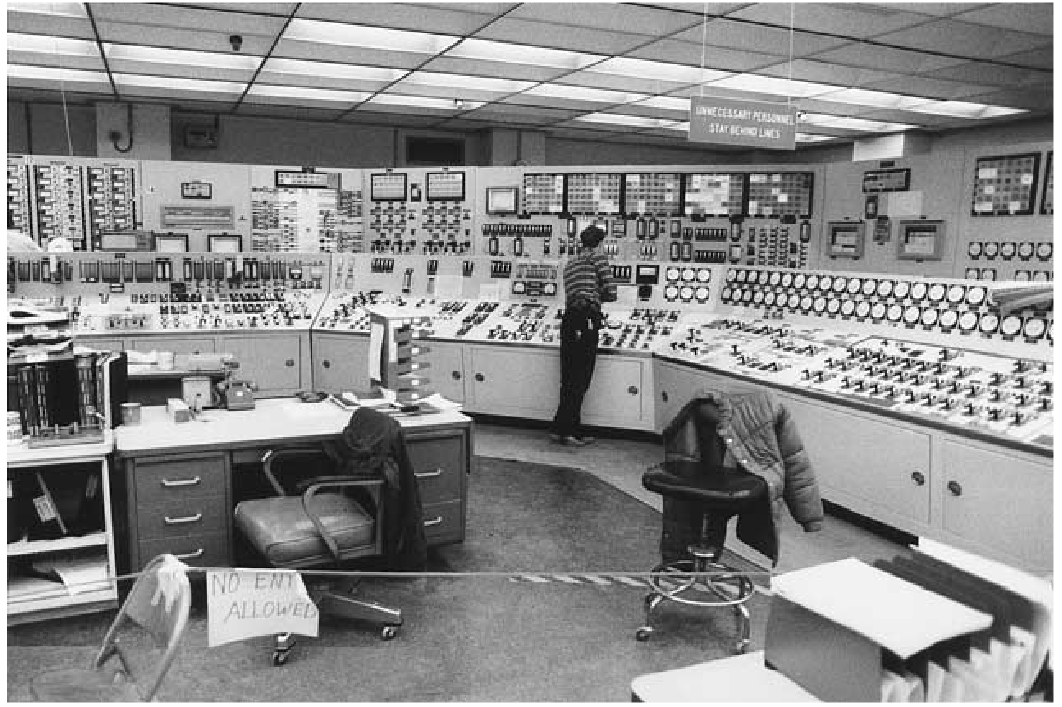
\includegraphics[width=0.75\textwidth]{tmicontrolroom.png}
\end{frame}

\begin{frame}{Chernobyl: Design and Assumption Failures}
  \subsubsection*{When Physics Fights Back}
  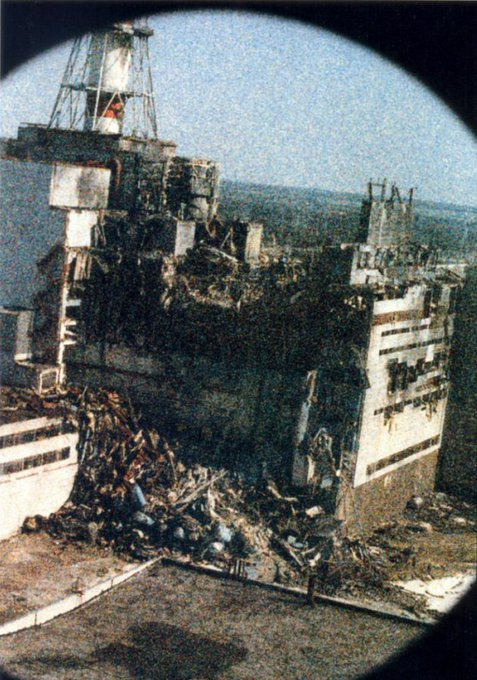
\includegraphics[width=0.6\textwidth]{chernobylafter.jpg}
  \speak{This photo shows the wreckage of Chernobyl's Reactor No.~4 just hours after the explosion. The graphite fire continued for days, spewing radiation across Europe \autocite{medvedev1991truth}.}
\end{frame}

\begin{frame}{Chernobyl: Design and Assumption Failures}
  \speak{Chernobyl's RBMK reactor had a positive void coefficient: as coolant boiled, reactivity rose. During a turbine coastdown test, this reactivity led to runaway power. A SCRAM—normally safe—made it worse, as control rods had graphite tips \autocite{iaea1992chernobyl}.}
  \begin{itemize}
    \item Unstable physics design, especially at low power
    \item Operators unaware of full core behavior
    \item Culture of secrecy delayed response and accountability
  \end{itemize}
\end{frame}

\begin{frame}{Fukushima: Nature and Neglect}
  \subsubsection*{Environmental Consequences}
  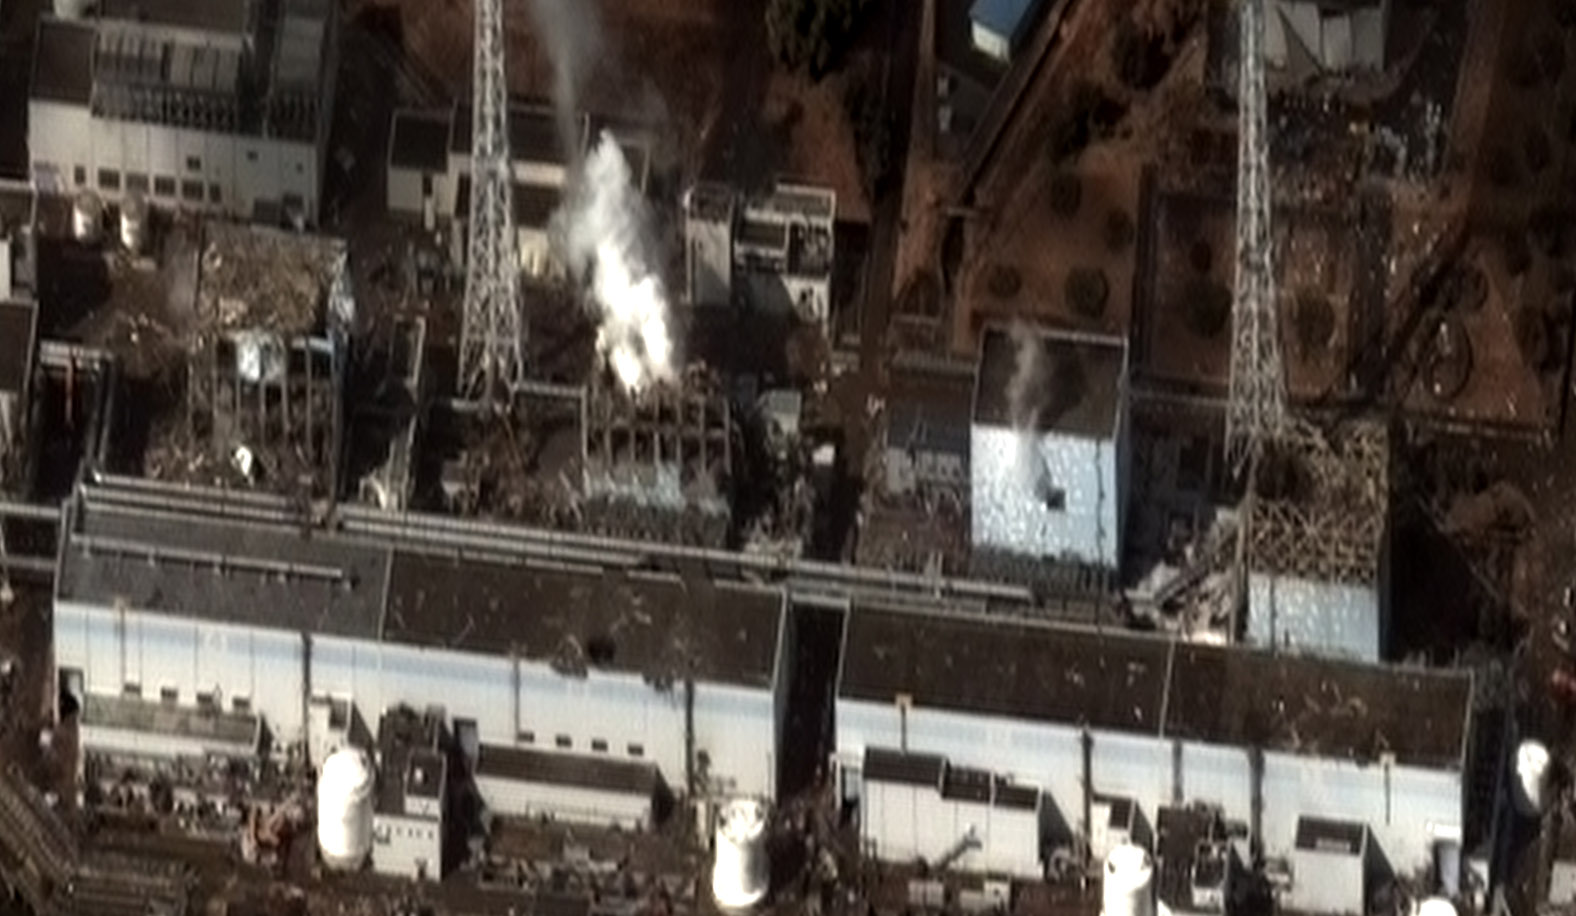
\includegraphics[width=0.75\textwidth]{fukushimaafter.jpg}
  \speak{Fukushima's tsunami flooded backup generators located in basements. This loss of power—called station blackout—disabled cooling, and all three operating units melted down \autocite{iaea_fukushima_report}.}
\end{frame}

\begin{frame}{Fukushima: Nature and Neglect}
  \speak{Though the reactors shutdown correctly, residual decay heat remained. Without cooling pumps, that heat caused core melt. Desperate engineers tried to wire car batteries together to read instrument panels \autocite{nrc_fukushima}.}
  \begin{itemize}
    \item Failure of backup power design
    \item Hydrogen explosions from vented zirconium reactions
    \item Ocean contamination and public trust fallout
  \end{itemize}
\end{frame}

\section{Human Factors}

\begin{frame}{Human Factors Engineering}
  \subsubsection*{Designing for the Operator}
  \speak{Modern control rooms use color-coded touch screens, redundancy, and full-scope training simulators. Human factors seeks to prevent misinterpretation and stress-based mistakes.}
  \begin{itemize}
    \item Cognitive load reduction
    \item Realistic training environments
    \item Alarm prioritization and filtering
  \end{itemize}
\end{frame}

\begin{frame}{Ethics of Automation}
  \subsubsection*{Keeping the Human in the Loop}
  \speak{Machines must serve—not replace—humans in nuclear operations. SCRAMs, alarms, logic interlocks: all must assume a trained operator will intervene. Ethical design means building for fallibility \autocite{mitocw_rbmkreview}.}
  \begin{itemize}
    \item Passive safety aids are essential
    \item But overtrust in automation can fail silently
    \item The human-in-the-loop design is non-negotiable
  \end{itemize}
\end{frame}

\section{Economic Challenges}

\begin{frame}{Aging Infrastructure and Waste}
  \subsubsection*{Legacy Risks}
  \speak{Beyond physics, the nuclear field is strained economically. Most U.S. plants were built pre-1980. Engineering supply chains have shrunk, and no long-term spent fuel site exists \autocite{wna2023chernobyl}.}
  \begin{itemize}
    \item On-site pools reaching capacity
    \item Dry cask storage: temporary fix
    \item Fewer experts entering the field
  \end{itemize}
\end{frame}

\begin{frame}{Modern Developments}
  \subsubsection*{New Hope: SMRs and Vogtle}
  \speak{Still, there is hope. Vogtle Units 3 and 4 in Georgia marked the first new reactors in decades. SMRs and molten salt reactors promise passive safety and easier siting \autocite{worldnuclear_vogtle}.}
  \begin{itemize}
    \item Factory assembly lowers construction risk
    \item Smaller cores, faster SCRAM times
    \item Potential role in green hydrogen and remote grids
  \end{itemize}
\end{frame}

\section{Conclusion}

\begin{frame}{Final Thoughts}
  \subsubsection*{Resilience Through Design}
  \speak{From SL-1 to Fukushima, the lesson is clear: safe nuclear power isn't just about neutrons. It's about people, design, and ethics. The atom, when split responsibly, can still light the world.}
  \begin{itemize}
    \item Prioritize human-machine partnerships
    \item Design with humility and feedback
    \item Build public trust through transparency
  \end{itemize}
\end{frame}

\begin{frame}{References}
  \nocite{*}
  \printbibliography
\end{frame}

\end{document}
